\documentclass[tikz,border=6pt]{standalone}
% Shared figure style for the Space Data Network whitepapers.
\usepackage{lmodern}
\usepackage[T1]{fontenc}
\usepackage{xcolor}
\usetikzlibrary{arrows.meta,positioning,calc,fit,backgrounds,matrix}
\hyphenpenalty=10000\exhyphenpenalty=10000
\definecolor{ink}{HTML}{1F2328}
\definecolor{rule}{HTML}{57606A}
\definecolor{panel}{HTML}{F3F4F6}
\definecolor{accent}{HTML}{D4880F}
\tikzset{
  every picture/.style={line width=0.6pt, draw=ink, text=ink, font=\small},
  box/.style={draw=ink, fill=panel, rounded corners=2pt, align=center, inner sep=5pt},
  plain/.style={draw=ink, fill=white, rounded corners=2pt, align=center, inner sep=5pt},
  title/.style={font=\bfseries\small},
  where/.style={font=\scriptsize\itshape, text=rule},
  note/.style={font=\footnotesize\itshape, text=rule},
  flow/.style={-{Stealth[length=2.2mm]}, draw=rule},
}

\begin{document}
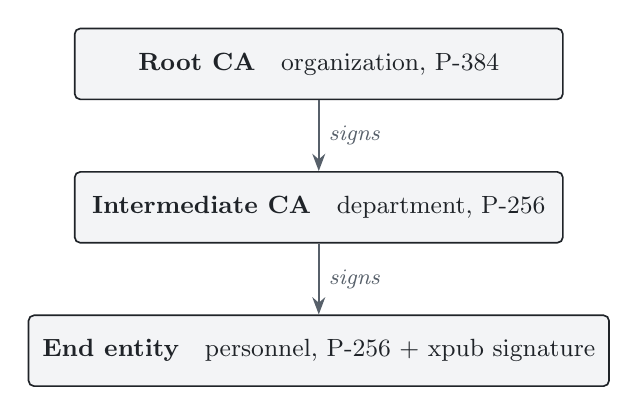
\begin{tikzpicture}[node distance=9mm, level/.style={box, minimum width=62mm, minimum height=9mm}]
\node[level] (root) {{\bfseries Root CA}\quad organization, P-384};
\node[level, below=of root] (mid) {{\bfseries Intermediate CA}\quad department, P-256};
\node[level, below=of mid] (leaf) {{\bfseries End entity}\quad personnel, P-256 + xpub signature};
\draw[flow] (root) -- node[right, note] {signs} (mid);
\draw[flow] (mid) -- node[right, note] {signs} (leaf);
\end{tikzpicture}
\end{document}
